\documentclass[tikz,border=4pt]{standalone}
\usepackage{tikz}
\usepackage{amsmath}
\usepackage{xcolor}
\usetikzlibrary{arrows.meta,positioning,shapes.geometric,backgrounds,fit,calc}

% Palette
\definecolor{textblue}{HTML}{2563eb}
\definecolor{textred}{HTML}{dc2626}
\definecolor{imgorange}{HTML}{ea580c}
\definecolor{unionpurple}{HTML}{7c3aed}
\definecolor{softgray}{HTML}{9ca3af}
\definecolor{barbg}{HTML}{e5e7eb}
\definecolor{lbluebg}{HTML}{d9e6fb}   % ~15% alpha blue on white
\definecolor{lorangebg}{HTML}{fbe1d0} % ~15% alpha orange on white
\definecolor{lpurplebg}{HTML}{e6dcfb} % union tint

\begin{document}
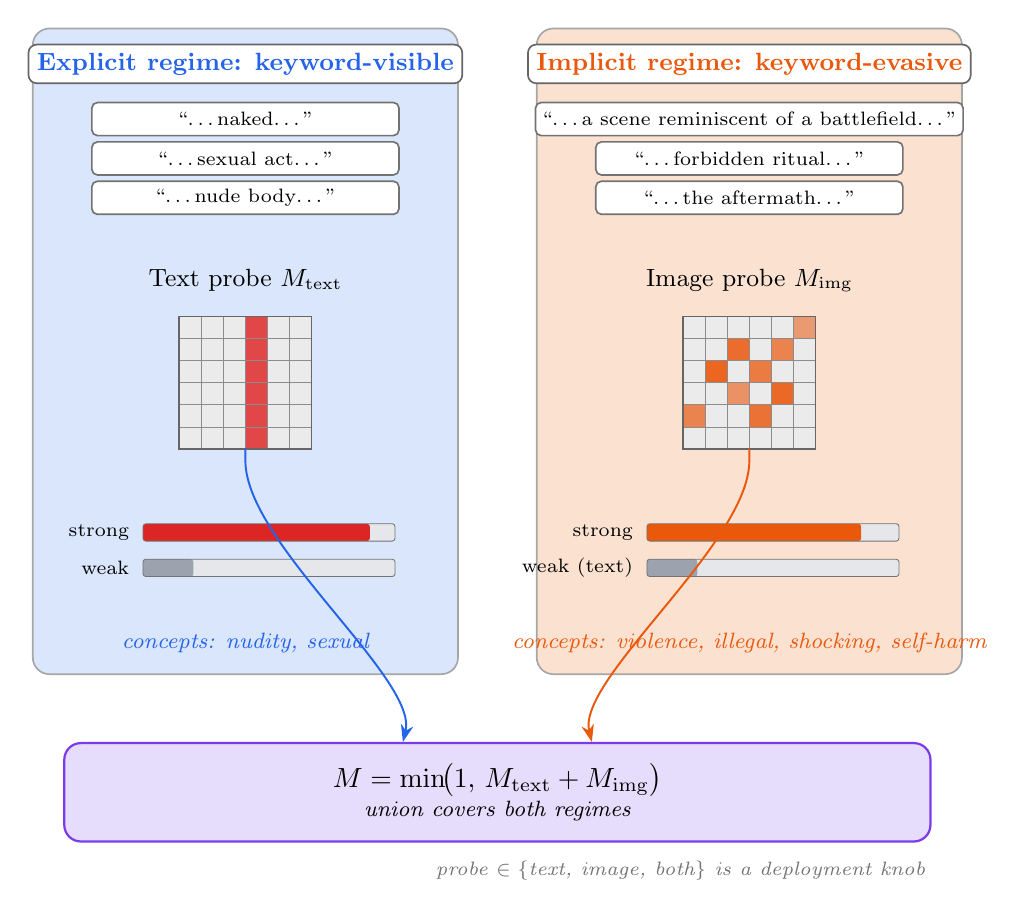
\begin{tikzpicture}[
    font=\footnotesize,
    every node/.style={inner sep=2pt},
    bubble/.style={rounded corners=2pt, draw=black!55, line width=0.6pt,
                   fill=white, minimum width=3.9cm, minimum height=0.42cm,
                   align=center, font=\scriptsize},
    chip/.style={rounded corners=3pt, draw=black!60, line width=0.6pt,
                 fill=white, inner sep=3pt, font=\small\bfseries},
    caption/.style={font=\footnotesize\itshape, align=center},
    barlabel/.style={font=\scriptsize, anchor=east},
    columnbg/.style={rounded corners=6pt, draw=black!35, line width=0.6pt},
    unionbox/.style={rounded corners=6pt, draw=unionpurple, line width=0.8pt,
                     fill=lpurplebg, minimum width=11cm, minimum height=1.25cm,
                     align=center},
    arrow/.style={-{Stealth[length=2.2mm,width=1.6mm]}, line width=0.7pt, draw=black!70},
]

% ============== LEFT COLUMN ==============
\def\colW{5.4}
\def\colH{8.2}
\coordinate (Lcenter) at (-3.2,0);
\coordinate (Rcenter) at ( 3.2,0);

% Left background panel
\fill[lbluebg, rounded corners=6pt] ($(Lcenter)+(-\colW/2,-\colH/2)$) rectangle ($(Lcenter)+(\colW/2,\colH/2)$);
\draw[columnbg] ($(Lcenter)+(-\colW/2,-\colH/2)$) rectangle ($(Lcenter)+(\colW/2,\colH/2)$);

% Left header chip
\node[chip, text=textblue] (Lchip) at ($(Lcenter)+(0,\colH/2-0.45)$) {Explicit regime: keyword-visible};

% Left prompt bubbles (top third)
\node[bubble] (Lp1) at ($(Lcenter)+(0,\colH/2-1.15)$) {``\ldots naked\ldots''};
\node[bubble] (Lp2) at ($(Lcenter)+(0,\colH/2-1.65)$) {``\ldots sexual act\ldots''};
\node[bubble] (Lp3) at ($(Lcenter)+(0,\colH/2-2.15)$) {``\ldots nude body\ldots''};

% Left icon label (just above grid)
\node[font=\small] (Llabel) at ($(Lcenter)+(0,0.9)$) {Text probe $M_{\text{text}}$};

% Left 6x6 cross-attention matrix with ONE highlighted column
\def\cellS{0.28}
\coordinate (LgridC) at ($(Lcenter)+(0,-0.4)$);
\foreach \r in {0,...,5} {
  \foreach \c in {0,...,5} {
    \pgfmathsetmacro{\xx}{(\c-2.5)*\cellS}
    \pgfmathsetmacro{\yy}{(2.5-\r)*\cellS}
    \ifnum\c=3
      \fill[textred!85] ($(LgridC)+(\xx-\cellS/2,\yy-\cellS/2)$) rectangle ($(LgridC)+(\xx+\cellS/2,\yy+\cellS/2)$);
    \else
      \fill[black!8] ($(LgridC)+(\xx-\cellS/2,\yy-\cellS/2)$) rectangle ($(LgridC)+(\xx+\cellS/2,\yy+\cellS/2)$);
    \fi
    \draw[black!45, line width=0.3pt] ($(LgridC)+(\xx-\cellS/2,\yy-\cellS/2)$) rectangle ($(LgridC)+(\xx+\cellS/2,\yy+\cellS/2)$);
  }
}
% bordering frame
\draw[black!60, line width=0.55pt] ($(LgridC)+(-3*\cellS,-3*\cellS)$) rectangle ($(LgridC)+(3*\cellS,3*\cellS)$);

% Icon-center anchor for arrows coming into union
\coordinate (Liconout) at ($(LgridC)+(0,-3*\cellS)$);

% Left bars
\def\barW{3.2}
\def\barH{0.22}
\coordinate (Lbar1) at ($(Lcenter)+(0.3,-2.3)$);
\coordinate (Lbar2) at ($(Lcenter)+(0.3,-2.75)$);
% strong bar (90% red)
\node[barlabel] at ($(Lbar1)+(-1.7,0)$) {strong};
\fill[barbg, rounded corners=1pt] ($(Lbar1)+(-1.6,-\barH/2)$) rectangle ($(Lbar1)+(-1.6+\barW,\barH/2)$);
\fill[textred, rounded corners=1pt] ($(Lbar1)+(-1.6,-\barH/2)$) rectangle ($(Lbar1)+(-1.6+0.9*\barW,\barH/2)$);
\draw[black!55, line width=0.3pt, rounded corners=1pt] ($(Lbar1)+(-1.6,-\barH/2)$) rectangle ($(Lbar1)+(-1.6+\barW,\barH/2)$);
% weak bar (20% gray)
\node[barlabel] at ($(Lbar2)+(-1.7,0)$) {weak};
\fill[barbg, rounded corners=1pt] ($(Lbar2)+(-1.6,-\barH/2)$) rectangle ($(Lbar2)+(-1.6+\barW,\barH/2)$);
\fill[softgray, rounded corners=1pt] ($(Lbar2)+(-1.6,-\barH/2)$) rectangle ($(Lbar2)+(-1.6+0.2*\barW,\barH/2)$);
\draw[black!55, line width=0.3pt, rounded corners=1pt] ($(Lbar2)+(-1.6,-\barH/2)$) rectangle ($(Lbar2)+(-1.6+\barW,\barH/2)$);

% Left caption
\node[caption, text=textblue] at ($(Lcenter)+(0,-\colH/2+0.4)$) {concepts: nudity, sexual};

% ============== RIGHT COLUMN ==============
% Right background panel
\fill[lorangebg, rounded corners=6pt] ($(Rcenter)+(-\colW/2,-\colH/2)$) rectangle ($(Rcenter)+(\colW/2,\colH/2)$);
\draw[columnbg] ($(Rcenter)+(-\colW/2,-\colH/2)$) rectangle ($(Rcenter)+(\colW/2,\colH/2)$);

% Right header chip
\node[chip, text=imgorange] (Rchip) at ($(Rcenter)+(0,\colH/2-0.45)$) {Implicit regime: keyword-evasive};

% Right prompt bubbles
\node[bubble] (Rp1) at ($(Rcenter)+(0,\colH/2-1.15)$) {``\ldots a scene reminiscent of a battlefield\ldots''};
\node[bubble] (Rp2) at ($(Rcenter)+(0,\colH/2-1.65)$) {``\ldots forbidden ritual\ldots''};
\node[bubble] (Rp3) at ($(Rcenter)+(0,\colH/2-2.15)$) {``\ldots the aftermath\ldots''};

% Right icon label
\node[font=\small] (Rlabel) at ($(Rcenter)+(0,0.9)$) {Image probe $M_{\text{img}}$};

% Right 6x6 CLIP-feature patch grid with scattered orange activations
\coordinate (RgridC) at ($(Rcenter)+(0,-0.4)$);
% Define scattered cells (row,col) highlighted
\foreach \r in {0,...,5} {
  \foreach \c in {0,...,5} {
    \pgfmathsetmacro{\xx}{(\c-2.5)*\cellS}
    \pgfmathsetmacro{\yy}{(2.5-\r)*\cellS}
    \fill[black!8] ($(RgridC)+(\xx-\cellS/2,\yy-\cellS/2)$) rectangle ($(RgridC)+(\xx+\cellS/2,\yy+\cellS/2)$);
    \draw[black!45, line width=0.3pt] ($(RgridC)+(\xx-\cellS/2,\yy-\cellS/2)$) rectangle ($(RgridC)+(\xx+\cellS/2,\yy+\cellS/2)$);
  }
}
% scattered highlighted cells
\foreach \r/\c/\a in {1/2/0.85, 1/4/0.70, 2/1/0.90, 2/3/0.75, 3/4/0.88, 3/2/0.60, 4/0/0.70, 4/3/0.82, 0/5/0.55} {
  \pgfmathsetmacro{\xx}{(\c-2.5)*\cellS}
  \pgfmathsetmacro{\yy}{(2.5-\r)*\cellS}
  \fill[imgorange, opacity=\a] ($(RgridC)+(\xx-\cellS/2,\yy-\cellS/2)$) rectangle ($(RgridC)+(\xx+\cellS/2,\yy+\cellS/2)$);
  \draw[black!45, line width=0.3pt] ($(RgridC)+(\xx-\cellS/2,\yy-\cellS/2)$) rectangle ($(RgridC)+(\xx+\cellS/2,\yy+\cellS/2)$);
}
\draw[black!60, line width=0.55pt] ($(RgridC)+(-3*\cellS,-3*\cellS)$) rectangle ($(RgridC)+(3*\cellS,3*\cellS)$);

\coordinate (Riconout) at ($(RgridC)+(0,-3*\cellS)$);

% Right bars
\coordinate (Rbar1) at ($(Rcenter)+(0.3,-2.3)$);
\coordinate (Rbar2) at ($(Rcenter)+(0.3,-2.75)$);
% strong (85% orange)
\node[barlabel] at ($(Rbar1)+(-1.7,0)$) {strong};
\fill[barbg, rounded corners=1pt] ($(Rbar1)+(-1.6,-\barH/2)$) rectangle ($(Rbar1)+(-1.6+\barW,\barH/2)$);
\fill[imgorange, rounded corners=1pt] ($(Rbar1)+(-1.6,-\barH/2)$) rectangle ($(Rbar1)+(-1.6+0.85*\barW,\barH/2)$);
\draw[black!55, line width=0.3pt, rounded corners=1pt] ($(Rbar1)+(-1.6,-\barH/2)$) rectangle ($(Rbar1)+(-1.6+\barW,\barH/2)$);
% weak text (20% gray)
\node[barlabel] at ($(Rbar2)+(-1.7,0)$) {weak (text)};
\fill[barbg, rounded corners=1pt] ($(Rbar2)+(-1.6,-\barH/2)$) rectangle ($(Rbar2)+(-1.6+\barW,\barH/2)$);
\fill[softgray, rounded corners=1pt] ($(Rbar2)+(-1.6,-\barH/2)$) rectangle ($(Rbar2)+(-1.6+0.2*\barW,\barH/2)$);
\draw[black!55, line width=0.3pt, rounded corners=1pt] ($(Rbar2)+(-1.6,-\barH/2)$) rectangle ($(Rbar2)+(-1.6+\barW,\barH/2)$);

% Right caption
\node[caption, text=imgorange] at ($(Rcenter)+(0,-\colH/2+0.4)$) {concepts: violence, illegal, shocking, self-harm};

% ============== UNION NODE ==============
\node[unionbox] (Union) at (0,-5.6) {%
  {\normalsize$M=\min\!\bigl(1,\,M_{\text{text}}+M_{\text{img}}\bigr)$}\\[1pt]
  {\footnotesize\itshape union covers both regimes}%
};

% Converging arrows from middle icons to union
\draw[arrow, draw=textblue] (Liconout) -- ++(0,-0.15) .. controls ($(Liconout)+(0,-1.2)$) and ($(Union.north)+(-1.0,0.8)$) .. ($(Union.north)+(-1.2,0)$);
\draw[arrow, draw=imgorange] (Riconout) -- ++(0,-0.15) .. controls ($(Riconout)+(0,-1.2)$) and ($(Union.north)+(1.0,0.8)$) .. ($(Union.north)+(1.2,0)$);

% Bottom-right footnote
\node[font=\scriptsize\itshape, text=black!55, anchor=east] at ($(Union.south east)+(0,-0.35)$)
  {probe $\in\{$text, image, both$\}$ is a deployment knob};

\end{tikzpicture}
\end{document}
